\documentclass[conference]{IEEEtran}

\usepackage[T1]{fontenc}
\usepackage[utf8]{inputenc}
\usepackage{amsmath}
\usepackage{booktabs}
\usepackage{graphicx}
\usepackage{microtype}
\usepackage{url}
\usepackage{xurl}
\usepackage[hidelinks]{hyperref}

\graphicspath{{./}{paper/}}

\title{DEEDY: A Thai-Centric Multi-Agent Framework for\\
Social-Media Marketing Campaign Analysis}

\author{\IEEEauthorblockN{Sawit Koseeyaumporn}
\IEEEauthorblockA{Department of Computer Engineering\\
King Mongkut's University of Technology Thonburi, Bangkok, Thailand\\
\texttt{sawit.kosee@kmutt.ac.th}}}

\begin{document}
\maketitle

\begin{abstract}
Social-media marketing campaigns generate large volumes of fast-moving,
context-dependent consumer reactions that are difficult to interpret with
sentiment classification alone. This paper presents DEEDY (Digital Environment
for Emergent Dynamics and Yield), a Thai-centric application and experimental
testbed for analyzing campaign response with large-language-model (LLM)
agents. For each campaign post, an Apify-based pipeline requests up to 1,000
publicly accessible comments from Facebook, Instagram, or TikTok, preserves
post and collection provenance, and produces synchronized raw and Thai-aware
analysis views. Campaign facts and approved context form a reality seed,
whereas observed reactions reserved for evaluation remain hidden from the
agents. DEEDY adapts MiroFish, an open-source multi-agent prediction engine
that converts seed documents into a GraphRAG-grounded world, generates actors,
runs OASIS social interactions, and supports report generation and post-run
inspection. The resulting application lets marketers examine how message
framing, audience composition, and platform mechanisms may shape simulated
reaction, diffusion, and narrative formation. We propose leakage-resistant
evaluation against held-out Thai comments using sentiment and stance
distribution distance, narrative coverage, response diversity, propagation
error, repeated runs, and native-Thai human assessment. DEEDY is positioned as
an exploratory campaign-planning and social-listening instrument, not as a
deterministic forecast of consumer behavior or a replacement for field
research.
\end{abstract}

\begin{IEEEkeywords}
LLM agents, social-media marketing, campaign analysis, social simulation, Thai
NLP, GraphRAG, MiroFish, Apify
\end{IEEEkeywords}

\section{Introduction}

Marketing campaigns on social media are not one-way messages. Consumers reply
to a campaign post, react to one another, repeat or contest emerging claims,
and carry interpretations across platform feeds. A favorable first response
may be displaced by complaints about price, product quality, brand conduct, or
the credibility of an influencer; conversely, a small positive narrative may
grow through recommendation and peer endorsement. Counting likes or assigning
sentiment to comments can summarize a snapshot, but it cannot by itself
represent the interaction process through which campaign narratives emerge.
Agent-based modeling (ABM) provides a bottom-up way to represent local exposure
and response decisions and observe their collective consequences
~\cite{macal2010tutorial}.

LLM agents extend ABM by allowing simulated actors to condition open-ended
actions on a profile, memory, retrieved evidence, feed context, and earlier
conversation. Generative Agents demonstrated memory-driven believable
behavior~\cite{park2023generative}, while Social Simulacra showed how generated
users and conversations can support social-computing prototypes
~\cite{park2022social}. Systems including $S^3$, OASIS, and GenSim subsequently
modeled social networks, recommendation, and multiple online actions at larger
scales~\cite{gao2023s3,yang2024oasis,tang2025gensim}. These capabilities suggest
a campaign-analysis application in which marketers can rehearse alternative
message framing, audience composition, and feed conditions before interpreting
the resulting differences as hypotheses for further testing.

\textbf{MiroFish} provides the application foundation for DEEDY. It converts
reality-seed documents into a GraphRAG-grounded environment, generates actors,
runs OASIS social interactions, and exposes the simulated world through report
and interaction agents~\cite{mirofish2026}. Its detailed workflow and validity
constraints are discussed in Related Work and the DEEDY framework.

Applying this workflow to Thai campaigns introduces two challenges. First,
Thai localization is more than translating an English prompt. Thai has no
obligatory whitespace between words, and campaign comments frequently combine
informal spelling, repeated characters, emoji, hashtags, transliterated
English, regional language, sarcasm, indirect disagreement, and culturally
specific politeness. Thai NLP resources and models have improved substantially
~\cite{arreerard2022survey,phatthiyaphaibun2023pythainlp,
lowphansirikul2021wangchanberta,pipatanakul2024typhoon2}, but cultural capability
remains a distinct evaluation target~\cite{kim2025thaicli}. Second, social data
collection is platform-dependent and incomplete. A reproducible study must
record which campaign post was queried, the collection time, the requested
limit, the returned count, and any access or visibility limitation.

A further methodological problem is that plausible campaign comments do not
prove behavioral fidelity. Demographically conditioned LLM samples can
approximate some human distributions~\cite{argyle2023out}, yet recent work finds
behavioral inconsistency across settings~\cite{mooney2025coherent}. Operational
validation against authentic comments also shows that matching surface form
can be separated from matching content~\cite{schwager2026conditioned}. For this
reason, campaign context needed to construct the simulation must be separated
from real consumer reactions used to test it, and stochastic conditions must
be repeated rather than judged from a single persuasive-looking run.

This paper presents \textbf{DEEDY}, a Thai-centric campaign-analysis
application that combines an Apify data-preparation pipeline, the MiroFish core,
and an explicit validation layer. Analysts provide campaign topics and public
post URLs from Facebook, Instagram, or TikTok. DEEDY requests up to 1,000
comments for each post, preserves provenance and conversation structure, and
separates campaign context from held-out consumer reactions. Within the
simulator, an analyst can compare a baseline campaign with counterfactual
message framing, actor composition, network structure, or recommendation
policy. The application reports where simulated and observed discourse agree
or diverge; it does not claim to forecast the choices of a specific person or
the Thai market as a whole.

Our contributions are threefold:
\begin{itemize}
    \item We define an end-to-end Thai campaign-data pipeline that uses Apify
    Actors to request up to 1,000 publicly accessible comments per campaign
    post, normalize cross-platform fields, preserve provenance, and produce
    Thai-aware views for analysis and simulation.
    \item We adapt the MiroFish/OASIS workflow to social-media marketing through
    campaign-grounded actor construction, Thai linguistic attributes,
    configurable campaign interventions, and auditable simulation outputs.
    \item We specify a leakage-resistant protocol that evaluates content,
    population, and dynamic correspondence against held-out Thai campaign
    reactions using repeated runs, native-Thai review, ablations, and
    uncertainty reporting.
\end{itemize}

\section{Related Work}

\subsection{Generative Agents and Social Simulation}

Traditional ABMs encode actor states and behavioral rules explicitly. LLM
agents complement this approach by generating context-dependent language and
actions, but introduce sensitivity to prompts, decoding, memory, and the shared
base model. Generative Agents use observation, reflection, and planning to
produce coherent-seeming routines~\cite{park2023generative}. $S^3$ connects LLM
perception and action to emotion, attitude, and a social network
~\cite{gao2023s3}. OASIS adds dynamic user and post state, follow/comment/repost
actions, and configurable interest- and popularity-based recommendation at
large agent scales~\cite{yang2024oasis}. GenSim emphasizes reusable scenario
functions and execution robustness~\cite{tang2025gensim}. DEEDY uses these
systems as infrastructure, but focuses on Thai campaign construction and
empirical validation rather than maximum population size.

\subsection{Grounding and Operational Validity}

MiroFish extracts entities and relations from uploaded reality seeds, stores
individual and collective memory in a graph-retrieval layer, generates OASIS
profiles, runs social platforms, and uses a report agent to query simulation
state~\cite{mirofish2026}. This workflow accelerates scenario construction, but
the generated report is still evidence about the simulated world, not evidence
that the world is valid. DEEDY therefore treats every simulation trace as a
hypothesis to compare with unseen observations.

Algorithmic fidelity compares LLM-generated and human subgroup distributions
~\cite{argyle2023out}. Conditioned Comment Prediction instead compares a
generated response with the authentic response a user left to a stimulus,
providing a closer operational test for social-media simulation
~\cite{schwager2026conditioned}. Validation of generative ABMs further benefits
from staged replication before novel counterfactual tests
~\cite{cross2025validating}. These ideas motivate DEEDY's campaign-level
holdout: material required to describe the campaign is available to agents,
whereas the consumer reactions used for scoring are not.

\subsection{Thai Online Language and Campaign Response}

Thai NLP remains comparatively resource-constrained, especially for informal
and downstream semantic tasks~\cite{arreerard2022survey}. PyThaiNLP provides
tokenization and other open Thai processing components
~\cite{phatthiyaphaibun2023pythainlp}; WangchanBERTa showed that Thai-specific
preprocessing and pretraining over news and social data matter
~\cite{lowphansirikul2021wangchanberta}; and Typhoon 2 extends Thai-optimized
models to instruction-following generation~\cite{pipatanakul2024typhoon2}.
ThaiCLI separately evaluates cultural and linguistic knowledge, highlighting
that general benchmark strength does not guarantee Thai cultural competence
~\cite{kim2025thaicli}.

Online affect is also contextual. Sarcasm can invert literal polarity, and
conversation history and user style improve its detection
~\cite{hazarika2018cascade}. This is important in Thai discussions, where
particles, quotation, exaggerated praise, wordplay, and shared cultural
references may signal stance indirectly. Accordingly, DEEDY keeps thread
context and raw text for evaluation and does not treat sentiment, stance, and
sarcasm as interchangeable labels.

\section{DEEDY Framework}

\begin{figure*}[t]
    \centering
    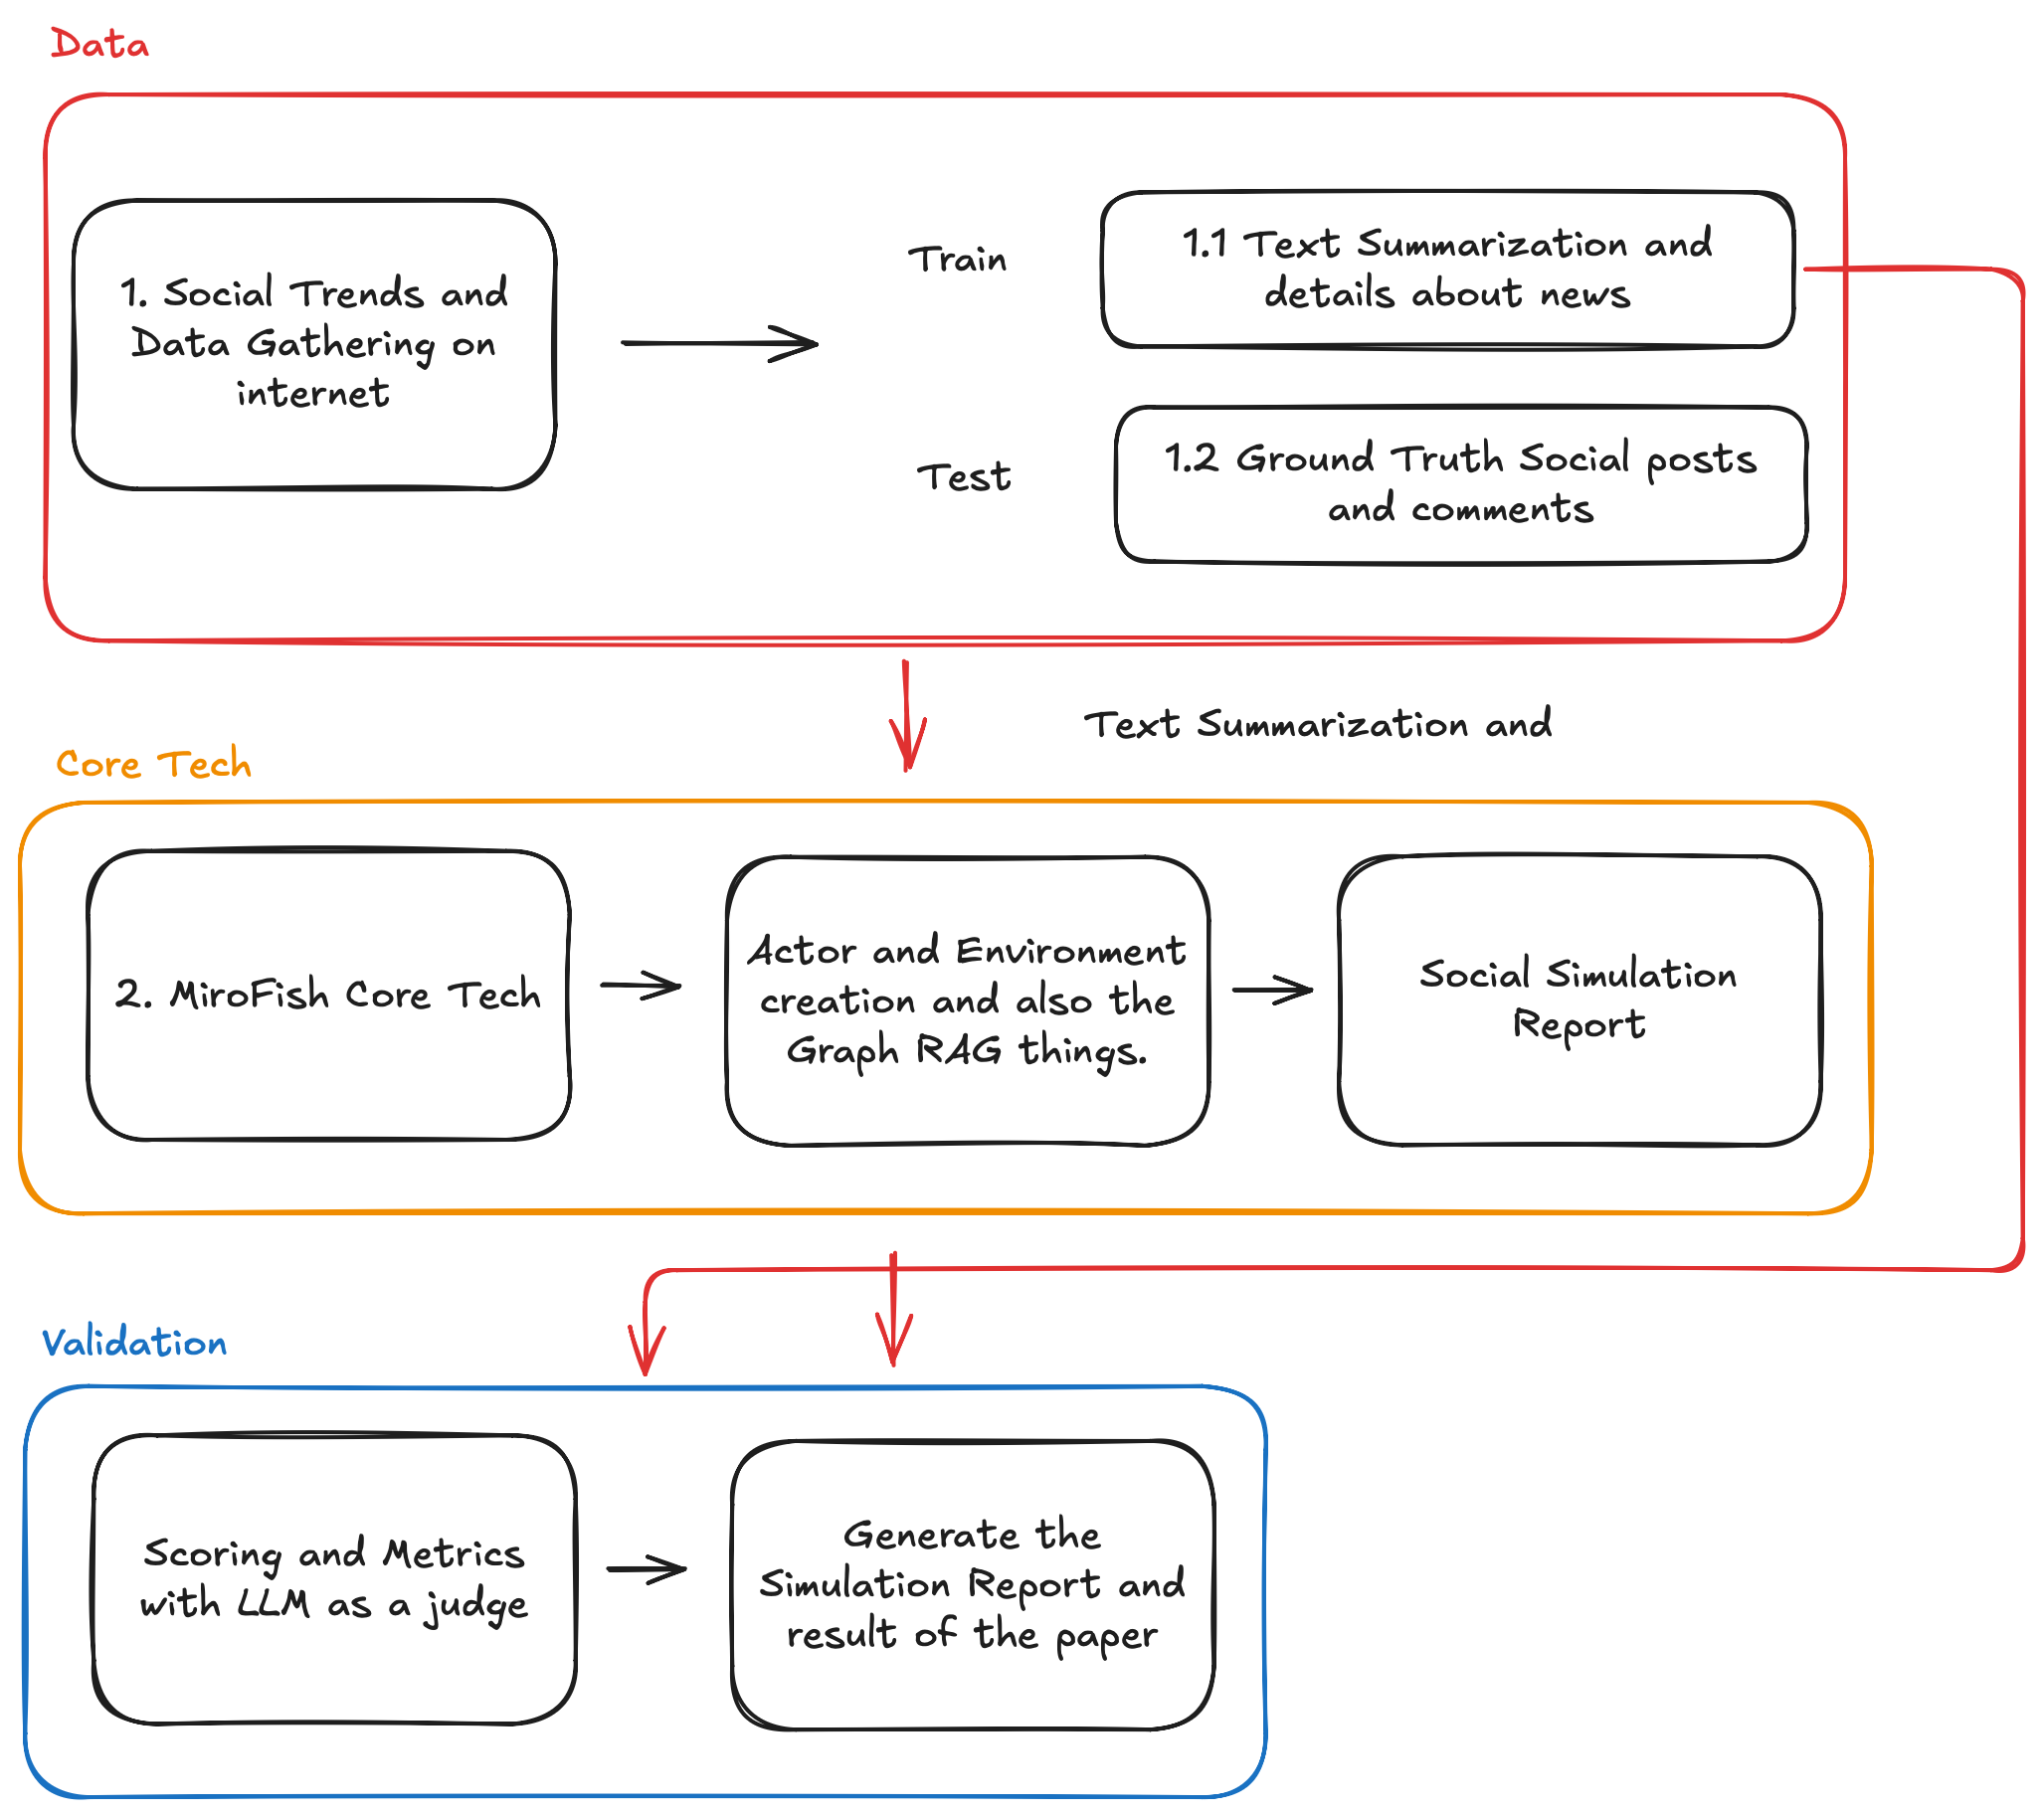
\includegraphics[width=0.78\textwidth]{system_arch.png}
    \caption{DEEDY application architecture. Thai campaign context and
    social-media data are
    separated into a scenario-construction stream and a held-out validation
    stream. The MiroFish core builds a graph-grounded environment and actors,
    runs social simulation, and exposes outputs for multi-level evaluation.}
    \label{fig:deedy-architecture}
\end{figure*}

\subsection{System Architecture Overview}

Figure~\ref{fig:deedy-architecture} organizes DEEDY into three layers. The
\emph{data layer} selects campaign posts, collects comments through Apify,
cleans, partitions, and annotates Thai campaign material. The \emph{core layer}
supplies the scenario summary to
MiroFish, which constructs a GraphRAG-backed world, creates heterogeneous
actors, executes social interactions, and generates a simulation report. The
\emph{validation layer} compares outputs with social posts and comments never
shown to the agents. Every derived artifact records a campaign identifier,
platform, post URL, provenance pointer, processing version, and experimental
split so that a score can be traced back to its evidence.

\subsection{Data Preparation Pipeline}

\subsubsection{Campaign Definition and Post Selection}

The input manifest \texttt{data/topic\_ref.json} defines one marketing campaign
per record through a campaign topic and a list of reference URLs. URLs may
refer to campaign posts, creator or influencer posts, news coverage, or public
community posts on Facebook, Instagram, and TikTok. Including more than the
brand's official account reduces the risk of measuring only an owned-audience
response. For an experimental release, the manifest is extended with a stable
campaign identifier, observation window, and source stratum. Each URL is
manually checked for campaign relevance and resolved to a canonical post before
collection. The sampling frame and inclusion rules are frozen before labels or
simulation outputs are inspected.

Campaign facts used to construct the simulated scenario are stored separately
from consumer reactions. The factual packet may include the campaign brief,
creative copy, product information, publication time, and dated public
reporting. It does not include the target comments later used for evaluation.
This distinction supports both retrospective campaign analysis and a stricter
prospective design in which only information available at campaign launch is
provided to the agents.

\subsubsection{Apify Comment Collection}
\label{sec:apify-collection}

DEEDY uses Apify Actors as the collection interface rather than a manually
maintained browser crawler. An Actor is a server-side program that accepts
structured input, executes as a recorded run, and writes results to an Apify
dataset accessible through the API or client libraries~\cite{apify2026actors}.
The implemented \texttt{apify\_crawler.py} detects the platform from each URL
and invokes \texttt{apify/facebook-comments-scraper},
\texttt{apify/instagram-comment-scraper}, or
\texttt{clockworks/tiktok-comments-scraper}. A platform adapter maps each
Actor's output into one common comment schema.

The collection unit is one social-media post. Under the revised protocol,
DEEDY launches an independent Actor query for every canonical post URL with a
requested limit of
\textbf{1,000 comments per post}. The limit is reset for each URL; it is not a
shared 1,000-comment budget for the campaign or topic. If a campaign contains
$m$ posts, the intended maximum is therefore
\begin{equation}
    N_{\max}=1{,}000m.
\end{equation}
The returned count may be lower when a post has fewer comments or when the
platform or Actor cannot expose every comment. Replies are configured
explicitly for each platform and are counted as separate records when returned.
Accordingly, ``1,000'' is a reproducible query cap, not a guarantee of 1,000
observations and not a claim of complete platform coverage.

\subsubsection{Normalization and Provenance}

Each returned item is validated and normalized to the fields
\texttt{topic}, \texttt{platform}, \texttt{post\_url},
\texttt{comment\_id}, anonymized \texttt{author}, \texttt{text},
\texttt{likes\_count}, \texttt{parent\_comment\_id}, and \texttt{timestamp}.
The parent identifier preserves reply structure when the Actor exposes it.
Missing values remain explicit rather than being inferred. Records without
comment text are excluded from content analysis but retained in run-level
quality-control counts when they represent Actor errors.

For reproducibility, a provenance manifest records the campaign and canonical
post identifiers, Actor identifier and version, complete run input, Apify run
and dataset identifiers, start and completion times, requested limit
(1,000), returned count, reply setting, error status, collection-code version,
and a checksum of the frozen raw export. Raw UTF-8 JSONL is immutable after a
successful run. Subsequent tables are derived from that snapshot and
de-duplicated first by platform comment identifier and then by normalized-text
similarity within a post. User names and platform identifiers are hashed or
removed before research analysis.

This design improves repeatability but does not turn the result into a random
sample. Search and post selection, platform ranking, deleted or moderated
comments, public visibility, geography, login state, and Actor behavior can all
affect what is returned. DEEDY therefore reports requested and observed counts
for every post and treats cross-platform comparisons as conditional on these
collection mechanisms.

\subsubsection{Thai-Aware Data Views}

The crawler preserves the Unicode comment text returned by each Actor in an
immutable JSONL view. The implemented
\texttt{convert\_comments\_to\_csv.py} then flattens nested post records into a
UTF-8-SIG table containing the campaign topic, comment, author, engagement,
platform, post, comment and parent identifiers, and timestamp. This second view
supports inspection and annotation without replacing the raw export.

DEEDY avoids aggressive text cleaning because emoji, Thai--English
code-mixing, orthographic repetition, hashtags, particles, negation, and
punctuation may carry campaign stance or affect. The analysis view standardizes
only encoding, line breaks, and whitespace; any additional transformation is
versioned and never overwrites the raw text. Thai tokenization is performed
only when a metric requires tokens, while character- and embedding-level
metrics are reported in parallel to reduce dependence on one segmentation
system.

\subsubsection{Evidence Split and Structured Weak Annotation}

For each campaign $e$, the collected evidence is partitioned before any model
summary is generated:
\begin{equation}
    D_e = S_e \;\dot\cup\; G_e,
\end{equation}
where $S_e$ is the scenario-construction set and $G_e$ is the held-out observed
reaction set. $S_e$ contains the campaign facts and context permitted at the
chosen simulation start time. $G_e$ contains comments and interactions that
the simulator must reproduce but never receives as memory. A post is assigned
wholly to one experimental role when post-level holdout is used; temporal
experiments instead apply a pre-registered timestamp cut. Comment identifiers,
quoted passages, and near duplicates cannot cross the boundary.

The frozen Apify records are passed to \texttt{llm\_prelabel.py} in bounded
batches. Three critique models independently assign a positive, neutral, or
negative label to each sampled comment and summarize campaign response. A
fourth model synthesizes their outputs into consensus sentiment labels, an
overall sentiment-direction analysis, recommended campaign next steps, and
possible business or operational changes. Exact sentiment counts are computed
from the consolidated comment-level labels rather than estimated from the
synthesis text. Additional evaluation labels for campaign stance, narrative,
purchase intent, and sarcasm are collected under the human-annotation protocol
rather than attributed to the current pre-labeling script.

These model outputs are \emph{weak pre-annotations}, not ground truth. Only a
summary derived from $S_e$ may enter MiroFish; labels or summaries derived from
$G_e$ are restricted to scoring and error analysis. Before the main experiment,
native Thai annotators review a frozen, source-stratified sample, adjudicate
disagreements, report Krippendorff's $\alpha$, and audit errors involving
sarcasm, code-mixing, indirect criticism, and platform source. This separation
prevents observed campaign reactions from leaking into agent memory.

\subsection{MiroFish Core Engine}

\subsubsection{Reality Seed and GraphRAG}

The scenario packet contains the campaign brief, creative message, dated
factual claims, named entities, brands, products, creators, and source-level
provenance from $S_e$.
MiroFish extracts an ontology and entity relations, then injects individual and
collective memories into its graph retrieval layer~\cite{mirofish2026}. A
retrieved memory attached to an agent action includes its supporting node or
source identifier. Unsupported details generated during graph construction are
marked as model assumptions and are not silently promoted to facts.

\subsubsection{Actor and Environment Construction}

Actors represent campaign-relevant audience roles justified by $S_e$, such as
existing customers, prospective customers, creator followers, brand advocates,
skeptics, journalists, community members, and bystanders. A profile separates
evidence-backed attributes from sampled attributes. The Thai adaptation adds
language register, Thai--English mixing rate, region or dialect only when
supported, politeness strategy, typical message length, activity rate,
campaign-interest prior, interests, and uncertainty. Demographic attributes
are not inferred from a single message. Population weights and network links
are sampled from documented priors and varied during sensitivity analysis
rather than presented as known facts.

The environment specifies platforms, action space, time step, feed capacity,
and recommendation mechanism. OASIS supplies posting, replying, reposting,
following, and browsing behavior with dynamic social and content state
~\cite{yang2024oasis}. DEEDY additionally records each exposure before an
action. This makes it possible to distinguish ``the agent never saw the
message'' from ``the agent saw and rejected the message,'' a necessary
distinction for interpreting diffusion failure.

\subsubsection{Thai Context in Perception and Action}

At each round, an actor retrieves relevant graph memory, observes a bounded
feed, updates a private state, and chooses an action or abstention. Prompts
require natural Thai consistent with the actor's register without demanding
caricatured dialect. They preserve uncertainty, allow silence, and prohibit
fabricated quotations or demographic claims. Conversation context is included
for reply generation because Thai stance and sarcasm may depend on an earlier
turn~\cite{hazarika2018cascade}. The language model is configurable: a
Thai-optimized model such as Typhoon 2 and a strong multilingual model are
compared under identical action rules rather than assuming either is superior.

\subsubsection{Simulation Outputs and Application Layer}

The core returns a machine-readable simulation log and a human-readable
campaign report. The
log contains agent state version, exposure set, retrieved evidence, selected
action, generated content, parent action, timestamp, and token/model settings.
The report summarizes dominant and minority narratives, sentiment and stance
trajectories, influential nodes, propagation paths, disagreement, and
unsupported claims. It also exposes uncertainty across runs.

The application allows a marketer or analyst to select a campaign, inspect the
scenario packet and graph, configure actor count and feed policy, run a
baseline or a counterfactual campaign message, compare it with held-out
observations, and drill down from an aggregate chart to the simulated posts
and evidence that produced it. Counterfactual reports compare conditions
inside the model; they are not presented as causal effects in the real Thai
consumer population.

\section{Experimental Design}

\subsection{Research Questions}

The evaluation is organized around four questions:
\begin{itemize}
    \item \textbf{RQ1 (Content):} Does DEEDY reproduce the sentiment, stance,
    narrative, and linguistic characteristics of held-out Thai reactions?
    \item \textbf{RQ2 (Population):} Does graph grounding and Thai adaptation
    improve aggregate correspondence without collapsing response diversity?
    \item \textbf{RQ3 (Dynamics):} Does the simulated interaction process match
    observed cascade size, shape, timing, and network structure?
    \item \textbf{RQ4 (Application):} Are campaign reports traceable, stable
    across repeated runs, and useful to Thai marketing analysts without
    overstating certainty?
\end{itemize}

\subsection{Dataset and Splitting Protocol}

The initial study will select campaigns with at least one usable factual
scenario packet and multiple public campaign-related posts. Before simulation,
the protocol freezes the required minimum returned-comment count, eligible
platforms, post-source strata, and missing-data rules. Apify then receives a
separate query for each post with a 1,000-comment limit as described in
Section~\ref{sec:apify-collection}. Posts returning fewer records are retained
when they satisfy the pre-registered minimum; the dataset never pads a short
thread by duplicating comments or borrowing another post's quota.

The unit of generalization is a \emph{campaign}, not an individual post or
comment. Prompt and model selection use development campaigns, and final
scores are reported on untouched test campaigns. Within a campaign, $S_e$ and
$G_e$ are separated either by a pre-registered timestamp or by whole post so
that a reaction thread cannot leak into both construction and evaluation.
Actor run inputs, query dates, returned counts, source strata, and split
assignments are frozen before weak annotation. This design supports
source-balanced analysis, temporal-drift checks, and sensitivity to
platform-specific public visibility.

Weak labels are independently reviewed by at least three native Thai
annotators using a codebook for three-way sentiment, campaign-specific stance,
sarcasm, and narrative membership. Annotators see necessary conversational
context but not whether a post is real or simulated during quality comparison.
Majority/adjudicated labels form the reference set, and Krippendorff's
$\alpha$ is reported for each task. User identifiers are hashed and quoted
examples are paraphrased unless publication is ethically justified.

\begin{table*}[t]
\caption{Planned experiments. Each condition is run with the same campaign
split, agent budget, round budget, and ten random seeds unless that factor is
varied.}
\label{tab:experiments}
\centering
\footnotesize
\begin{tabular}{@{}p{0.16\textwidth}p{0.31\textwidth}p{0.43\textwidth}@{}}
\toprule
Experiment & Conditions & Primary purpose \\
\midrule
Exp. 1: Grounding & DEEDY seed-only; ungrounded LLM agents; deliberately leaky
all-source upper bound & Test whether held-out correspondence comes from the
scenario pipeline rather than parametric knowledge or target leakage. \\
Exp. 2: Thai adaptation & Full Thai adaptation; translated/unadapted MiroFish;
normalization without context features & Measure sentiment/stance distance,
narrative coverage, Thai quality, sarcasm, code-mixing, and diversity. \\
Exp. 3: Core model & Thai-optimized LLM; matched multilingual LLM; simple
non-generative ABM baseline & Separate the contribution of the language model
from the graph, population, and platform mechanisms. \\
Exp. 4: Social mechanism & Chronological, popularity, and interest feeds;
observed versus random network; multiple population sizes & Test cascade,
polarization, herding, and sensitivity to platform assumptions. \\
Exp. 5: Application & Baseline campaign versus one pre-registered
message-framing
counterfactual; report with versus without uncertainty/evidence links & Assess
traceability, analyst usefulness, and whether presentation changes trust. \\
\bottomrule
\end{tabular}
\end{table*}

\subsection{Metrics}

\subsubsection{Content and Population Correspondence}

Let $P_G^y$ and $P_S^y$ be observed and simulated distributions for label
$y\in\{\text{sentiment},\text{stance},\text{narrative}\}$. Distributional
correspondence is measured with Jensen--Shannon distance:
\begin{equation}
 d_{\mathrm{JS}}(P_G^y,P_S^y)=
 \sqrt{\tfrac{1}{2}D_{\mathrm{KL}}(P_G^y\Vert M)+
 \tfrac{1}{2}D_{\mathrm{KL}}(P_S^y\Vert M)},
\end{equation}
where $M=(P_G^y+P_S^y)/2$. Lower is better and the square-root form is bounded.
Macro-F1 is also reported when simulated posts are matched to a conditioned
stimulus or stance target.

Narrative correspondence is measured in two ways. First, Thai annotators map
posts to a campaign-specific narrative codebook and we compare coverage and
prevalence. Second, multilingual BERTScore measures semantic similarity between
generated and observed response sets~\cite{zhang2020bertscore}. Embedding-based
scores are treated as complementary because semantic proximity need not imply
the same stance. Diversity is reported using Distinct-1/2, Self-BLEU, unique
narrative count, lexical entropy, length distribution, and pairwise embedding
distance. High correspondence accompanied by diversity collapse is considered
a failure.

Polarization is measured from the stance distribution and interaction graph.
We report normalized stance entropy, between-group versus within-group
interaction, and modularity after fixing the community-detection procedure.
Population statistics are computed per run and then aggregated across
campaigns, so campaigns with many selected posts do not automatically dominate
the result.

\subsubsection{Temporal and Network Correspondence}

For trace-enriched campaigns, cumulative activity curves are aligned to the
campaign-post publication time. We report normalized root-mean-square error
(NRMSE) and dynamic time
warping distance, together with cascade scale, maximum depth, maximum breadth,
structural virality, time to 50\% of final activity, and peak-time error. OASIS
uses scale, depth, breadth, and propagation-curve error in its own validation
~\cite{yang2024oasis}; DEEDY adds exposure-conditioned action rates and Thai
content labels.

Observed and simulated interaction graphs are compared by degree and cascade-
size distributions using the two-sample Kolmogorov--Smirnov statistic, plus
clustering coefficient, reciprocity, assortativity, modularity, and the share
of cross-stance replies. These metrics are omitted, rather than imputed, when
the source platform does not expose the required trace.

\subsubsection{Thai Quality and Report Evaluation}

Native Thai raters score blinded real and simulated posts on a five-point scale
for naturalness, contextual coherence, stance consistency, pragmatic and
cultural appropriateness, and persona consistency. Sarcasm precision, recall,
and F1 are evaluated separately. Report claims are scored for evidence
traceability: the proportion of factual claims linked to scenario evidence or
simulation events, unsupported-claim rate, contradiction rate, and coverage of
minority narratives.

An LLM judge may assist high-volume screening, but cannot be the sole quality
measure. Pair order is swapped, output identity is hidden, the judge must cite
the supplied evidence before scoring, and its agreement with Thai raters is
reported. These controls address known position bias in LLM-as-a-judge
evaluation~\cite{shi2024judging}.

\subsection{Execution and Statistical Analysis}

All stochastic conditions use ten seeds initially; a power analysis on pilot
variance determines the final number. Model name and revision, prompts,
temperature, top-$p$, agent count, network seed, recommendation parameters,
round count, stopping rule, and token cost are frozen before the test set is
opened. We report medians and 95\% bootstrap confidence intervals across
campaigns. Paired conditions use a campaign-level permutation test or Wilcoxon
signed-rank test with Holm correction. Effect sizes accompany $p$-values.

The main comparison is the full DEEDY pipeline versus translated/unadapted
MiroFish. Component ablations remove graph retrieval, Thai context features,
thread context, or observed population weights one at a time. The deliberately
leaky condition in Table~\ref{tab:experiments} is never a valid system result;
it is a diagnostic ceiling showing how much apparent performance can be gained
by exposing held-out reactions.

\subsection{Acceptance Criteria for the Application}

Before results are observed, the study will set minimum criteria: (i) full
pipeline completion and provenance for every scored run; (ii) statistically
lower sentiment/stance Jensen--Shannon distance than the unadapted baseline;
(iii) no significant diversity collapse relative to held-out posts; (iv) Thai
quality above the midpoint with acceptable annotator agreement; (v) report
unsupported-claim rate below a pre-registered threshold; and (vi), for
trace-enriched campaigns, improvement on at least two cascade metrics without
material degradation on the others. Failure remains a reportable result and
defines the application's operating boundary.

\section{Limitations and Ethical Considerations}

The campaign corpus is a convenience sample of manually selected public posts
from Facebook, Instagram, and TikTok and cannot represent the Thai population
or each platform's users. Apify Actors can retrieve only comments exposed by
their collection mechanism; the 1,000-comment request may therefore return
fewer records and may reflect ranking, geography, login state, moderation,
deletion, platform change, or Actor failure. Coordinated activity and bots may
also bias observed response. Requested and returned counts, Actor versions,
and failures must consequently accompany every result. Even lightweight
normalization can alter pragmatic cues, so linguistic claims must be checked
against the paired raw view.

Personas can reproduce stereotypes even when generated from real traces.
DEEDY therefore avoids inferring sensitive attributes from isolated posts,
reports subgroup results only where data and ethics permit, and presents
regional or dialect attributes as uncertain rather than essential. Public
availability does not remove privacy risk: identifiers must be hashed, raw
text access restricted, quotations minimized, and collection reviewed against
platform terms and institutional research-ethics requirements.

Finally, LLM agents share training data, architecture, and prompt conventions;
agreement between them may reflect a common model prior rather than social
consensus. Counterfactual campaign findings are conditional on the scenario,
actor sampling, network, recommender, and model version. DEEDY is therefore an
instrument for exploratory comparison and hypothesis generation, not a
replacement for campaign experiments, customer research, surveys, or
participatory research with Thai communities.

\section{Conclusion and Future Work}

\emph{Placeholder---to be completed after the data pipeline, MiroFish core,
and experiments are finalized. The final conclusion will summarize measured
findings, supported application claims, failure cases, and next steps without
introducing results that are not reported in the paper.}

\bibliographystyle{IEEEtran}
\bibliography{deedy_references}

\end{document}
